\documentclass[a4paper, 12pt]{article}

\usepackage{hyperref}
\usepackage[warn]{mathtext}
\usepackage[utf8]{inputenc}
\usepackage[T2A]{fontenc}
\usepackage[english,russian]{babel}
\usepackage{multirow}
\usepackage{amsmath,amsfonts,amssymb,amsthm,mathtools}
\usepackage{indentfirst}
\DeclareSymbolFont{T2Aletters}{T2A}{cmr}{m}{it}
\usepackage{ gensymb }
\mathtoolsset{showonlyrefs=true}
\usepackage{euscript}
\usepackage{mathrsfs}
\usepackage[left=2cm,right=2cm,top=2cm,bottom=2cm]{geometry}
\usepackage{graphicx}
\usepackage{wrapfig}
\usepackage[rgb]{xcolor}
\hypersetup{
colorlinks=true,
urlcolor=blue
}


\title{Лабораторная работа}
\author{Гисич Арсений Б03-102}
\date{2022}

\begin{document}

	\begin{center}
		{\large МОСКОВСКИЙ ФИЗИКО-ТЕХНИЧЕСКИЙ ИНСТИТУТ (НАЦИОНАЛЬНЫЙ ИССЛЕДОВАТЕЛЬСКИЙ УНИВЕРСИТЕТ)}
	\end{center}
	\vspace{5 cm}
	{\Large
		\begin{center}
			{\bf Лабораторная работа 3.3.1}\\[0.2 cm]
			Измерение удельного заряда электрона методами магнитной фокусировки и магнетрона
		\end{center}
	}
	\vspace{4 cm}
	\begin{flushright}
		{\Large Выполнил: \\
			\vspace{0.2 cm}
			Гисич Арсений \\
			\vspace{0.2 cm}
			Б03-102 \\}
	\end{flushright}
	\vspace{9 cm}
	\begin{center}
		Долгопрудный\\[0.1 cm]
		2022
	\end{center}
\thispagestyle{empty}

\section{Аннотация}

В данной работе было определено отношение заряда электрона к его массе методами магнитной фокусировки и магнетрона.

\section{Метод магнитной фокусировки}

\subsection{Теоретические сведения}

Здесь удельный заряд электрона определяется по формуле
\begin{equation}
\dfrac{e}{m_e} = \dfrac{8\pi^2V}{l^2} \left(\dfrac{n^2}{B_{\text{ф}}^2} \right),
\end{equation}
где $V$ - ускоряющий потенциал в электронной трубке, $l$ - путь электрона, $B_{\text{ф}}$ - фокусирующее поле, $n$ - номер фокуса.

\subsection{Методика измерений}

\begin{wrapfigure}{l}{0.2\textwidth}
  \begin{center}
    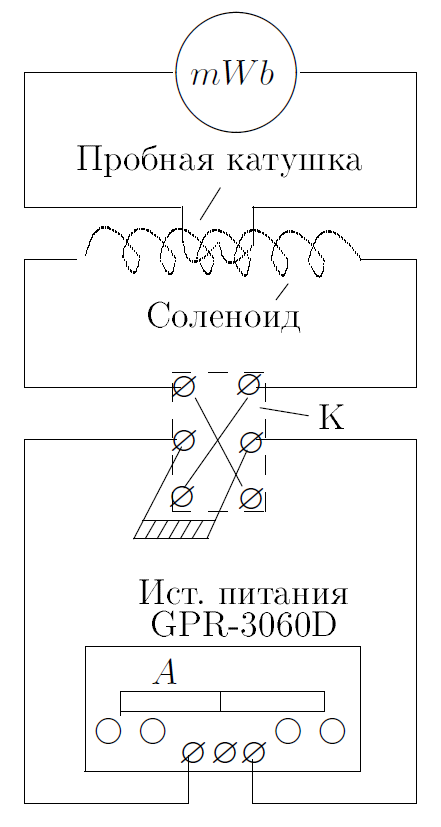
\includegraphics[width = 0.2\textwidth]{1.png}
  \end{center}
  \caption{Схема установки}
\end{wrapfigure}
Основной частью установки является электронный осциллограф, трубка которого вынута и установлена в длинном соленоиде, создающим магнитное поле. Напряжение на отклоняющие пластины и питание подводятся к трубке многожильным кабелем.

Пучок электронов, вылетающих из катода с разными скоростями, ускоряется анодным напряжением. Пропустив пучок сквозь две узкие диафрагмы, можно выделить электроны с практически одинаковой продольной скоростью. Небольшое переменное напряжение, поступающее с клеммы "Контрольный сигнал" осциллографа на отклоняющие пластины, изменяет только поперечную составляющую скорости. При увеличении магнитного поля линия на экране стягивается в точку, а затем снова удлиняется. 

Магнитное поле создается постоянным током, величина которого регулируется ручками источника питания и измеряется амперметром. Ключ служит для изменения направления поля в соленоиде.

Величина магнитного поля определяется с помощью милливеберметра.

На точность результатов может влиять внешнее магнитное поле, особенно продольное. 

Измерения магнитного поля с помощью милливеберметра обычно проводятся в предварительных опыта: при отключении ключа устанавливается связь между силой тока и индукцией магнитного поля в соленоиде. 

\subsection{Используемое оборудование}

\begin{enumerate}
    \item электронно-лучевая трубка;
    \item солениод;
    \item регулируемый источник постоянного тока;
    \item вольтметр;
    \item магнитометр.
\end{enumerate}

\section{Метод магнетрона}

\subsection{Теоретические сведения}

Здесь удельный заряд электрона определяется по формуле
\begin{equation}
\dfrac{e}{m_e} = \dfrac{8V_a}{B_{\text{кр}}^2r_a^2},
\end{equation}
где $V_a$ - анодное напряжение, $B_{\text{кр}}$ - критическое поле, $r_a$ - радиус анода.

\subsection{Методика измерений}

\begin{wrapfigure}{l}{0.3\textwidth}
  \begin{center}
    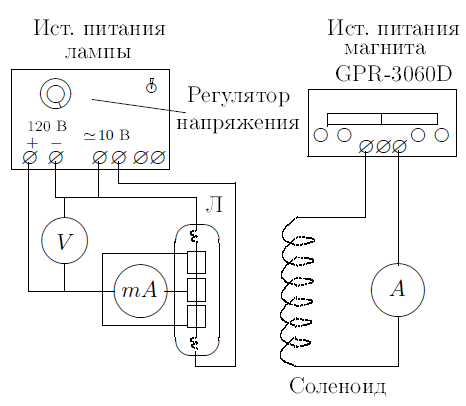
\includegraphics[width = 0.3\textwidth]{2.png}
  \end{center}
  \caption{Схема установки}
\end{wrapfigure}
Два крайних цилиндра изолированы от среднего небольшими зазорами и используются для устранения краевых эффектов на торцах среднего цилиндра, ток с которого используется при измерениях. В качестве катода используется тонкая вольфрамовая проволока. Катод разогревается переменным током, отбираемым от стабилизированного источника питания. 

С этого же источника на анод лампы подается напряжение, регулируемое с помощью потенциометра и измеряемое вольтметром.

Индукция магнитного поля в соленоиде рассчитывается по току $I_m$, протекающему через обмотку соленоида. Коэффициент пропорциональности между ними указан в установке.

Лампа закреплена в соленоиде. Магнитное поле в соленоиде создается постоянным током, сила которого регулируется ручками источника питания и измеряется амперметром.

\subsection{Используемое оборудование}

\begin{enumerate}
    \item электронная лампа с цилиндрическим анодом;
    \item регулируемый источник постоянного тока;
    \item соленоид;
    \item вольтметр;
    \item 2 амперметра.
\end{enumerate}

\section{Результаты измерений и обработка данных}



\section{Обсуждение результатов и выводы}

В данной работе исследовалась зависимость сдвига фаз в цепи переменного тока от его активного сопротивления при различных параметрах контура. По результатам измерений для RC-цепи зависимость существенно отклоняется от теоретической, а для RL-цепи согласуется с теорией. Это может быть вызвано плохим контактом соединительных проводов, небольшим количеством измерений или особенностями оборудования в экспериментальной установке.

Добротность исследованной RCL-цепи не превысила 10 при нулевом сопротивлении магазина, а при подключении дополнительного сопротивления и вовсе близка к единице. Это позволяет сделать вывод о том, что данная установка мало подходит для изучения собственных слабозатухающих колебаний в RCL-цепи, так как затухание колебаний в такой цепи будет слишком быстрым. Однако проведённый опыт показал, что полученные значения добротности достаточны для применимости использованной установки при исследовании вынужденных колебаний.

При исследовании фазовращателя рассчитанное теоретически сопротивление магазина, при котором сдвиг фаз между входным и выходным напряжениями равен $\pi/2$, близко от побобранной экспериментально, что согласуется с теорией.

\end{document}